% Options for packages loaded elsewhere
\PassOptionsToPackage{unicode}{hyperref}
\PassOptionsToPackage{hyphens}{url}
%
\documentclass[
]{article}
\usepackage{amsmath,amssymb}
\usepackage{iftex}
\ifPDFTeX
  \usepackage[T1]{fontenc}
  \usepackage[utf8]{inputenc}
  \usepackage{textcomp} % provide euro and other symbols
\else % if luatex or xetex
  \usepackage{unicode-math} % this also loads fontspec
  \defaultfontfeatures{Scale=MatchLowercase}
  \defaultfontfeatures[\rmfamily]{Ligatures=TeX,Scale=1}
\fi
\usepackage{lmodern}
\ifPDFTeX\else
  % xetex/luatex font selection
\fi
% Use upquote if available, for straight quotes in verbatim environments
\IfFileExists{upquote.sty}{\usepackage{upquote}}{}
\IfFileExists{microtype.sty}{% use microtype if available
  \usepackage[]{microtype}
  \UseMicrotypeSet[protrusion]{basicmath} % disable protrusion for tt fonts
}{}
\makeatletter
\@ifundefined{KOMAClassName}{% if non-KOMA class
  \IfFileExists{parskip.sty}{%
    \usepackage{parskip}
  }{% else
    \setlength{\parindent}{0pt}
    \setlength{\parskip}{6pt plus 2pt minus 1pt}}
}{% if KOMA class
  \KOMAoptions{parskip=half}}
\makeatother
\usepackage{xcolor}
\usepackage[margin=1in]{geometry}
\usepackage{color}
\usepackage{fancyvrb}
\newcommand{\VerbBar}{|}
\newcommand{\VERB}{\Verb[commandchars=\\\{\}]}
\DefineVerbatimEnvironment{Highlighting}{Verbatim}{commandchars=\\\{\}}
% Add ',fontsize=\small' for more characters per line
\usepackage{framed}
\definecolor{shadecolor}{RGB}{248,248,248}
\newenvironment{Shaded}{\begin{snugshade}}{\end{snugshade}}
\newcommand{\AlertTok}[1]{\textcolor[rgb]{0.94,0.16,0.16}{#1}}
\newcommand{\AnnotationTok}[1]{\textcolor[rgb]{0.56,0.35,0.01}{\textbf{\textit{#1}}}}
\newcommand{\AttributeTok}[1]{\textcolor[rgb]{0.13,0.29,0.53}{#1}}
\newcommand{\BaseNTok}[1]{\textcolor[rgb]{0.00,0.00,0.81}{#1}}
\newcommand{\BuiltInTok}[1]{#1}
\newcommand{\CharTok}[1]{\textcolor[rgb]{0.31,0.60,0.02}{#1}}
\newcommand{\CommentTok}[1]{\textcolor[rgb]{0.56,0.35,0.01}{\textit{#1}}}
\newcommand{\CommentVarTok}[1]{\textcolor[rgb]{0.56,0.35,0.01}{\textbf{\textit{#1}}}}
\newcommand{\ConstantTok}[1]{\textcolor[rgb]{0.56,0.35,0.01}{#1}}
\newcommand{\ControlFlowTok}[1]{\textcolor[rgb]{0.13,0.29,0.53}{\textbf{#1}}}
\newcommand{\DataTypeTok}[1]{\textcolor[rgb]{0.13,0.29,0.53}{#1}}
\newcommand{\DecValTok}[1]{\textcolor[rgb]{0.00,0.00,0.81}{#1}}
\newcommand{\DocumentationTok}[1]{\textcolor[rgb]{0.56,0.35,0.01}{\textbf{\textit{#1}}}}
\newcommand{\ErrorTok}[1]{\textcolor[rgb]{0.64,0.00,0.00}{\textbf{#1}}}
\newcommand{\ExtensionTok}[1]{#1}
\newcommand{\FloatTok}[1]{\textcolor[rgb]{0.00,0.00,0.81}{#1}}
\newcommand{\FunctionTok}[1]{\textcolor[rgb]{0.13,0.29,0.53}{\textbf{#1}}}
\newcommand{\ImportTok}[1]{#1}
\newcommand{\InformationTok}[1]{\textcolor[rgb]{0.56,0.35,0.01}{\textbf{\textit{#1}}}}
\newcommand{\KeywordTok}[1]{\textcolor[rgb]{0.13,0.29,0.53}{\textbf{#1}}}
\newcommand{\NormalTok}[1]{#1}
\newcommand{\OperatorTok}[1]{\textcolor[rgb]{0.81,0.36,0.00}{\textbf{#1}}}
\newcommand{\OtherTok}[1]{\textcolor[rgb]{0.56,0.35,0.01}{#1}}
\newcommand{\PreprocessorTok}[1]{\textcolor[rgb]{0.56,0.35,0.01}{\textit{#1}}}
\newcommand{\RegionMarkerTok}[1]{#1}
\newcommand{\SpecialCharTok}[1]{\textcolor[rgb]{0.81,0.36,0.00}{\textbf{#1}}}
\newcommand{\SpecialStringTok}[1]{\textcolor[rgb]{0.31,0.60,0.02}{#1}}
\newcommand{\StringTok}[1]{\textcolor[rgb]{0.31,0.60,0.02}{#1}}
\newcommand{\VariableTok}[1]{\textcolor[rgb]{0.00,0.00,0.00}{#1}}
\newcommand{\VerbatimStringTok}[1]{\textcolor[rgb]{0.31,0.60,0.02}{#1}}
\newcommand{\WarningTok}[1]{\textcolor[rgb]{0.56,0.35,0.01}{\textbf{\textit{#1}}}}
\usepackage{longtable,booktabs,array}
\usepackage{calc} % for calculating minipage widths
% Correct order of tables after \paragraph or \subparagraph
\usepackage{etoolbox}
\makeatletter
\patchcmd\longtable{\par}{\if@noskipsec\mbox{}\fi\par}{}{}
\makeatother
% Allow footnotes in longtable head/foot
\IfFileExists{footnotehyper.sty}{\usepackage{footnotehyper}}{\usepackage{footnote}}
\makesavenoteenv{longtable}
\usepackage{graphicx}
\makeatletter
\newsavebox\pandoc@box
\newcommand*\pandocbounded[1]{% scales image to fit in text height/width
  \sbox\pandoc@box{#1}%
  \Gscale@div\@tempa{\textheight}{\dimexpr\ht\pandoc@box+\dp\pandoc@box\relax}%
  \Gscale@div\@tempb{\linewidth}{\wd\pandoc@box}%
  \ifdim\@tempb\p@<\@tempa\p@\let\@tempa\@tempb\fi% select the smaller of both
  \ifdim\@tempa\p@<\p@\scalebox{\@tempa}{\usebox\pandoc@box}%
  \else\usebox{\pandoc@box}%
  \fi%
}
% Set default figure placement to htbp
\def\fps@figure{htbp}
\makeatother
\usepackage{svg}
\setlength{\emergencystretch}{3em} % prevent overfull lines
\providecommand{\tightlist}{%
  \setlength{\itemsep}{0pt}\setlength{\parskip}{0pt}}
\setcounter{secnumdepth}{-\maxdimen} % remove section numbering
\usepackage{bookmark}
\IfFileExists{xurl.sty}{\usepackage{xurl}}{} % add URL line breaks if available
\urlstyle{same}
\hypersetup{
  hidelinks,
  pdfcreator={LaTeX via pandoc}}

\author{}
\date{\vspace{-2.5em}}

\begin{document}

{
\setcounter{tocdepth}{2}
\tableofcontents
}
\section{Evaluación y Predicción de la Madurez Digital en Instituciones
de Educación Superior mediante Técnicas de Analítica de
Datos}\label{evaluaciuxf3n-y-predicciuxf3n-de-la-madurez-digital-en-instituciones-de-educaciuxf3n-superior-mediante-tuxe9cnicas-de-analuxedtica-de-datos}

\textbf{Autores:} Víctor Santos-Logroño \textbf{Filiación:} Escuela
Politécnica Nacional, Departamento de Automatización y Control
Industrial \textbf{Contacto:}
\href{mailto:victor.santos@epn.edu.ec}{\nolinkurl{victor.santos@epn.edu.ec}}

\section{1. Introducción}\label{introducciuxf3n}

La transformación digital se ha consolidado como uno de los pilares
estratégicos para la sostenibilidad, competitividad y capacidad de
innovación de las instituciones de educación superior (IES). En un
entorno caracterizado por la automatización de procesos, la integración
de sistemas, el uso intensivo de datos y la necesidad de ofrecer
servicios educativos flexibles y eficientes, comprender el estado actual
y la proyección futura de la madurez digital institucional se vuelve
fundamental.

La madurez digital no solo implica la adopción de tecnologías, sino
también la existencia de una visión estratégica, capacidades
organizacionales, liderazgo directivo, inversión sostenida, cultura de
innovación y una adecuada gestión del cambio. Su evaluación permite:

\begin{itemize}
\item
  Identificar brechas entre el nivel actual y el deseado.
\item
  Priorizar inversiones en infraestructura, talento humano y sistemas.
\item
  Comprender los factores que impulsan o limitan la transformación
  digital.
\item
  Modelar escenarios futuros para la toma de decisiones basadas en
  evidencia.
\end{itemize}

En este contexto, el estudio de la madurez digital requiere no solo el
análisis estático de indicadores, sino también el desarrollo de modelos
predictivos que permitan anticipar la evolución institucional en función
de múltiples factores organizacionales, tecnológicos y culturales.

\section{2. Disponibilidad limitada de datos públicos sobre madurez
digital en
IES}\label{disponibilidad-limitada-de-datos-puxfablicos-sobre-madurez-digital-en-ies}

A pesar de la creciente importancia de la transformación digital en IES,
la disponibilidad de datasets públicos que permitan estudiar este
fenómeno de forma cuantitativa y reproducible es todavía muy limitada.
La mayoría de iniciativas de evaluación digital se encuentran en
informes privados, auditorías internas o estudios sectoriales cuyos
datos no son compartidos por motivos de confidencialidad, competitividad
o protección institucional.En consecuencia:

\begin{itemize}
\item
  Acceso limitado a repositorios públicos con métricas longitudinales de
  madurez digital.
\item
  Los datasets disponibles son principalmente transversales, con un solo
  levantamiento por institución.
\item
  La diversidad metodológica entre estudios impide la combinación de
  bases de datos.
\end{itemize}

Dentro de este contexto, el dataset \emph{Raw OpenData Digital-Survey
HEI Germany} disponible en
\href{https://doi.org/10.5281/zenodo.6383770}{\pandocbounded{\includesvg[keepaspectratio]{https://zenodo.org/badge/DOI/10.5281/zenodo.6383770.svg}}}
representa una de las pocas iniciativas de datos abiertos sobre madurez
digital institucional en educación superior a nivel global. Su valor
reside principalmente en su alcance, nivel de detalle y metodología. Sin
embargo, como se explica a continuación, sus características
estructurales lo vuelven inadecuado para ciertos tipos de análisis
avanzados, particularmente modelos predictivos supervisados o
evaluaciones longitudinales.

\subsection{\texorpdfstring{2.1 Análisis técnico del dataset \emph{Raw
OpenData Digital-Survey HEI Germany} y evaluación de su
idoneidad}{2.1 Análisis técnico del dataset Raw OpenData Digital-Survey HEI Germany y evaluación de su idoneidad}}\label{anuxe1lisis-tuxe9cnico-del-dataset-raw-opendata-digital-survey-hei-germany-y-evaluaciuxf3n-de-su-idoneidad}

Antes de aplicar cualquier técnica de análisis avanzada es indispensable
evaluar la calidad, estructura y capacidad informativa del dataset
disponible. En estudios de madurez digital, la calidad del dato adquiere
una importancia crítica, ya que la predicción del nivel futuro de
digitalización y la identificación de patrones institucionales dependen
directamente de la variabilidad interna, la completitud y la riqueza
informacional de los ítems evaluados.

Dado que la encuesta \emph{Raw OpenData Digital-Survey HEI Germany} fue
publicada de forma agregada y parcialmente anonimizada, es necesario
establecer, mediante métricas objetivas, si este dataset posee las
condiciones estadísticas mínimas para sostener un análisis predictivo
robusto.

\subsubsection{2.1.1 Proporción global de valores
faltantes}\label{proporciuxf3n-global-de-valores-faltantes}

Una condición mínima para aplicar técnicas multivariantes o modelos
supervisados es disponer de un volumen suficiente de datos observados.
Los valores faltantes (NA) reducen el tamaño de la muestra efectiva,
generan sesgos y obligan a aplicar imputaciones que disminuyen la
fiabilidad del análisis. Por ello, se evalúa la proporción global de NA
en el dataset RAW.

\begin{Shaded}
\begin{Highlighting}[]
\CommentTok{\# Descarga automática del dataset RAW}
\ControlFlowTok{if}\NormalTok{ (}\SpecialCharTok{!}\FunctionTok{dir.exists}\NormalTok{(}\StringTok{"data"}\NormalTok{)) }\FunctionTok{dir.create}\NormalTok{(}\StringTok{"data"}\NormalTok{)}

\NormalTok{url\_raw }\OtherTok{\textless{}{-}} \StringTok{"https://zenodo.org/records/6383770/files/Raw\_OpenData\_Digital{-}Survey\_HEI{-}Germany.csv?download=1"}
\NormalTok{destino }\OtherTok{\textless{}{-}} \StringTok{"data/Raw\_OpenData\_Digital{-}Survey\_HEI{-}Germany.csv"}

\ControlFlowTok{if}\NormalTok{ (}\SpecialCharTok{!}\FunctionTok{file.exists}\NormalTok{(destino)) \{}
  \FunctionTok{download.file}\NormalTok{(url\_raw, }\AttributeTok{destfile =}\NormalTok{ destino, }\AttributeTok{mode =} \StringTok{"wb"}\NormalTok{)}
\NormalTok{\}}

\FunctionTok{file.info}\NormalTok{(destino)}
\end{Highlighting}
\end{Shaded}

\begin{verbatim}
##                                                     size isdir mode
## data/Raw_OpenData_Digital-Survey_HEI-Germany.csv 1777720 FALSE  660
##                                                                mtime
## data/Raw_OpenData_Digital-Survey_HEI-Germany.csv 2025-12-10 14:43:44
##                                                                ctime
## data/Raw_OpenData_Digital-Survey_HEI-Germany.csv 2025-12-10 14:43:44
##                                                                atime     uid
## data/Raw_OpenData_Digital-Survey_HEI-Germany.csv 2025-12-10 14:43:45 3193170
##                                                    gid    uname       grname
## data/Raw_OpenData_Digital-Survey_HEI-Germany.csv 10001 r3127634 rstudio-user
\end{verbatim}

\begin{Shaded}
\begin{Highlighting}[]
\CommentTok{\# Carga del dataset RAW y limpieza inicial}
\FunctionTok{library}\NormalTok{(dplyr)}
\end{Highlighting}
\end{Shaded}

\begin{verbatim}
## 
## Attaching package: 'dplyr'
\end{verbatim}

\begin{verbatim}
## The following objects are masked from 'package:stats':
## 
##     filter, lag
\end{verbatim}

\begin{verbatim}
## The following objects are masked from 'package:base':
## 
##     intersect, setdiff, setequal, union
\end{verbatim}

\begin{Shaded}
\begin{Highlighting}[]
\FunctionTok{library}\NormalTok{(tidyr)}
\FunctionTok{library}\NormalTok{(janitor)}
\end{Highlighting}
\end{Shaded}

\begin{verbatim}
## 
## Attaching package: 'janitor'
\end{verbatim}

\begin{verbatim}
## The following objects are masked from 'package:stats':
## 
##     chisq.test, fisher.test
\end{verbatim}

\begin{Shaded}
\begin{Highlighting}[]
\FunctionTok{library}\NormalTok{(ggplot2)}
\FunctionTok{library}\NormalTok{(entropy)}

\CommentTok{\# Lectura correcta del archivo RAW (usa separador ";")}
\NormalTok{datos\_raw }\OtherTok{\textless{}{-}} \FunctionTok{read.csv}\NormalTok{(destino,}
\AttributeTok{sep =} \StringTok{";"}\NormalTok{,}
\AttributeTok{header =} \ConstantTok{TRUE}\NormalTok{,}
\AttributeTok{stringsAsFactors =} \ConstantTok{FALSE}\NormalTok{,}
\AttributeTok{encoding =} \StringTok{"UTF{-}8"}\NormalTok{)}

\CommentTok{\# Limpieza de nombres de columnas}
\NormalTok{datos\_raw }\OtherTok{\textless{}{-}} \FunctionTok{clean\_names}\NormalTok{(datos\_raw)}

\CommentTok{\# Reemplazo de códigos técnicos por NA}
\NormalTok{datos\_raw }\OtherTok{\textless{}{-}}\NormalTok{ datos\_raw }\SpecialCharTok{|\textgreater{}}
\FunctionTok{mutate}\NormalTok{(}\FunctionTok{across}\NormalTok{(}\FunctionTok{everything}\NormalTok{(),}
\SpecialCharTok{\textasciitilde{}} \FunctionTok{ifelse}\NormalTok{(. }\SpecialCharTok{\%in\%} \FunctionTok{c}\NormalTok{(}\SpecialCharTok{{-}}\DecValTok{1}\NormalTok{, }\SpecialCharTok{{-}}\DecValTok{2}\NormalTok{, }\StringTok{"{-}1"}\NormalTok{, }\StringTok{"{-}2"}\NormalTok{), }\ConstantTok{NA}\NormalTok{, .)))}

\CommentTok{\# Vista general de dimensiones}
\FunctionTok{dim}\NormalTok{(datos\_raw)}
\end{Highlighting}
\end{Shaded}

\begin{verbatim}
## [1]  445 1371
\end{verbatim}

\begin{Shaded}
\begin{Highlighting}[]
\CommentTok{\# Vista preliminar de las primeras columnas}
\FunctionTok{head}\NormalTok{(datos\_raw[, }\DecValTok{1}\SpecialCharTok{:}\DecValTok{10}\NormalTok{])}
\end{Highlighting}
\end{Shaded}

\begin{verbatim}
##   v_id     v_date v1 v2 v3   v4 v5 v6    v7 v8
## 1    1 01.02.2022  2 NA NA   NA NA NA       NA
## 2    2 31.01.2022  2 NA NA   NA NA NA       NA
## 3    3 31.01.2022  1  2 10 2577 NA NA large NA
## 4    4 31.01.2022  4 NA NA   NA NA NA       NA
## 5    5 31.01.2022 NA NA NA   NA NA NA       NA
## 6    6 31.01.2022 NA NA NA   NA NA NA       NA
\end{verbatim}

\begin{Shaded}
\begin{Highlighting}[]
\CommentTok{\# Proporción de NA por variable}
\NormalTok{prop\_na }\OtherTok{\textless{}{-}}\NormalTok{ datos\_raw }\SpecialCharTok{\%\textgreater{}\%}
  \FunctionTok{summarise}\NormalTok{(}\FunctionTok{across}\NormalTok{(}\FunctionTok{everything}\NormalTok{(), }\SpecialCharTok{\textasciitilde{}} \FunctionTok{mean}\NormalTok{(}\FunctionTok{is.na}\NormalTok{(.)))) }\SpecialCharTok{\%\textgreater{}\%}
  \FunctionTok{pivot\_longer}\NormalTok{(}\FunctionTok{everything}\NormalTok{(), }\AttributeTok{names\_to =} \StringTok{"variable"}\NormalTok{, }\AttributeTok{values\_to =} \StringTok{"prop\_na"}\NormalTok{)}

\CommentTok{\# Promedio global}
\NormalTok{mean\_na\_global }\OtherTok{\textless{}{-}} \FunctionTok{mean}\NormalTok{(prop\_na}\SpecialCharTok{$}\NormalTok{prop\_na)}
\NormalTok{mean\_na\_global}
\end{Highlighting}
\end{Shaded}

\begin{verbatim}
## [1] 0.8466976
\end{verbatim}

El cálculo muestra que el dataset \emph{Raw OpenData Digital-Survey HEI
Germany} presenta una proporción promedio de 84.7\% de valores
faltantes, lo que indica un nivel crítico de incompletitud. Con un
porcentaje tan elevado, la mayoría de variables carece de suficientes
datos para permitir análisis multivariados, clustering o modelos
predictivos confiables, ya que solo alrededor del 15\% de la información
esperada está realmente disponible.

Este grado de ausencia sugiere una encuesta con fuerte heterogeneidad en
la respuesta (no todas las instituciones contestan los mismos bloques),
generando una matriz extremadamente dispersa que imposibilita aplicar
técnicas estadísticas estándar.

\subsubsection{2.1.2 Variedad y estabilidad informativa de las
variables}\label{variedad-y-estabilidad-informativa-de-las-variables}

La calidad de un dataset para análisis multivariante o predictivo
depende no solo de la ausencia de valores faltantes, sino también del
grado de información útil que contienen sus variables. En encuestas de
madurez digital, es habitual que muchas preguntas no sean respondidas o
presenten patrones de respuesta demasiado homogéneos, lo cual impide
extraer estructura estadística.

Por ello, se evalúa la \emph{entropía de Shannon} de cada variable, una
medida estándar que cuantifica cuánta información aporta:

\begin{itemize}
\item
  Entropía baja: la variable casi no cambia, aporta poca señal.
\item
  Entropía alta: la variable tiene variación significativa, es
  potencialmente útil.
\end{itemize}

Este paso permite identificar si el dataset posee suficientes variables
informatívamente estables como para justificar análisis posteriores.

\begin{Shaded}
\begin{Highlighting}[]
\CommentTok{\# Seleccionar solo variables categóricas o numéricas convertidas a factor}
\NormalTok{datos\_entropia }\OtherTok{\textless{}{-}}\NormalTok{ datos\_raw }\SpecialCharTok{|\textgreater{}}
\FunctionTok{mutate}\NormalTok{(}\FunctionTok{across}\NormalTok{(}\FunctionTok{everything}\NormalTok{(), as.factor))}

\CommentTok{\# Función para calcular entropía con manejo de NA}
\NormalTok{calc\_entropia }\OtherTok{\textless{}{-}} \ControlFlowTok{function}\NormalTok{(x)\{}
\NormalTok{x }\OtherTok{\textless{}{-}}\NormalTok{ x[}\SpecialCharTok{!}\FunctionTok{is.na}\NormalTok{(x)]}
\ControlFlowTok{if}\NormalTok{ (}\FunctionTok{length}\NormalTok{(}\FunctionTok{unique}\NormalTok{(x)) }\SpecialCharTok{\textless{}=} \DecValTok{1}\NormalTok{) }\FunctionTok{return}\NormalTok{(}\DecValTok{0}\NormalTok{)}
\NormalTok{p }\OtherTok{\textless{}{-}} \FunctionTok{prop.table}\NormalTok{(}\FunctionTok{table}\NormalTok{(x))}
\FunctionTok{entropy}\NormalTok{(p, }\AttributeTok{unit=}\StringTok{"log2"}\NormalTok{)}
\NormalTok{\}}

\NormalTok{entropias }\OtherTok{\textless{}{-}} \FunctionTok{sapply}\NormalTok{(datos\_entropia, calc\_entropia)}

\CommentTok{\# Convertir a dataframe ordenado}
\NormalTok{df\_entropia }\OtherTok{\textless{}{-}} \FunctionTok{data.frame}\NormalTok{(}
\AttributeTok{variable =} \FunctionTok{names}\NormalTok{(entropias),}
\AttributeTok{entropia =}\NormalTok{ entropias}
\NormalTok{) }\SpecialCharTok{|\textgreater{}} \FunctionTok{arrange}\NormalTok{(}\FunctionTok{desc}\NormalTok{(entropia))}

\FunctionTok{head}\NormalTok{(df\_entropia, }\DecValTok{15}\NormalTok{)}
\end{Highlighting}
\end{Shaded}

\begin{verbatim}
##                        variable entropia
## v_id                       v_id 8.797662
## v_action_4438_1 v_action_4438_1 8.797662
## v_duration           v_duration 8.788673
## v_runtime             v_runtime 8.283205
## v4                           v4 7.046946
## v_pagetime1         v_pagetime1 6.060440
## v_pagetime2         v_pagetime2 5.799106
## v_pagetime3         v_pagetime3 5.708727
## v1028                     v1028 5.350342
## v30                         v30 5.325413
## v1027                     v1027 5.247022
## v29                         v29 5.227461
## v627                       v627 5.218943
## v626                       v626 5.159727
## v_score                 v_score 5.053601
\end{verbatim}

Los resultados muestran que solo un número muy reducido de variables del
dataset presenta valores de entropía moderados o altos, lo que indica
que la gran mayoría de ítems carece de variabilidad suficiente para
capturar patrones informativos útiles.

Como se observa en la tabla anterior, las variables con mayor entropía
corresponden casi exclusivamente a campos operativos como v\_id,
v\_action\_4438\_1, v\_duration, v\_runtime y medidas de pagetime, es
decir, variables técnicas asociadas al sistema de captura, no a
constructos de madurez digital. Este comportamiento revela que las
variables verdaderamente vinculadas al contenido de la encuesta son en
su mayoría constantes, casi vacías o presentan una estructura
extremadamente dispersa.

\subsubsection{2.1.3 Justificación del no uso del
dataset}\label{justificaciuxf3n-del-no-uso-del-dataset}

El análisis exploratorio realizado sobre el dataset \emph{Raw OpenData
Digital-Survey HEI Germany} permite concluir que, pese a su relevancia
como iniciativa pública de medición de madurez digital, su versión RAW
carece de las condiciones estadísticas mínimas para sustentar un estudio
multivariante o predictivo con estándares académicos avanzados.

En primer lugar, la presencia extrema de valores perdidos y la baja
completitud transversal impiden construir una matriz de información
estable y limitan severamente la posibilidad de aplicar técnicas de
reducción de dimensionalidad o clasificación supervisada. Además, la
evaluación de entropía muestra que la variabilidad efectiva del dataset
se concentra en un número muy reducido de variables técnicas, mientras
que los ítems conceptuales asociados a madurez digital presentan
variabilidad nula o marginal, imposibilitando identificar patrones
institucionales con significado analítico.

A partir de estos hallazgos, se concluye que el dataset no es adecuado
como base empírica para los objetivos del estudio, que requieren una
estructura de datos consistente, informativa y con variabilidad
suficiente para modelar niveles de madurez digital y predecir escenarios
futuros. No obstante, \textbf{este análisis no es un ejercicio fallido},
por el contrario, evidencia con claridad cuáles son las limitaciones
metodológicas de los instrumentos existentes y orienta la construcción
de una nueva encuesta estructurada, diseñada específicamente para evitar
estos problemas.

\section{3. Diseño conceptual de una encuesta multiactor para modelar la
madurez digital
institucional}\label{diseuxf1o-conceptual-de-una-encuesta-multiactor-para-modelar-la-madurez-digital-institucional}

El análisis previo del \emph{Raw OpenData Digital-Survey HEI Germany}
evidenció limitaciones importantes para su uso directo en un estudio
orientado a la modelización predictiva de la madurez digital
institucional. En particular, se observó una combinación poco favorable
de alta proporción de valores ausentes, baja variabilidad efectiva en un
número considerable de ítems y ausencia de una variable objetivo
claramente interpretable como indicador de madurez digital.

Ante esta situación, se plantea el diseño de un instrumento propio que
permita generar un conjunto de datos específicamente estructurado para
análisis multivariante y modelos supervisados, incorporando
explícitamente los requerimientos de calidad de datos identificados en
el diagnóstico inicial. Un principio central de este diseño es la
consideración de la transformación digital como un fenómeno sociotécnico
que involucra a todos los grupos de interés de la IES.

En esta sección se define la arquitectura conceptual de la encuesta, los
actores que participan en la medición y los bloques temáticos que deben
ser incluidos para asegurar la posterior construcción de indicadores de
madurez digital y variables explicativas de calidad.

\subsection{3.1 Actores involucrados en la
medición}\label{actores-involucrados-en-la-mediciuxf3n}

Dado que la madurez digital institucional no se limita a la
disponibilidad tecnológica, sino que integra dimensiones de estrategia,
cultura organizacional y experiencia del usuario, la encuesta se plantea
con un enfoque multiactor. Por lo que se proponen cuatro grupos de
respuesta:

\begin{itemize}
\tightlist
\item
  \emph{Autoridades} (rector, vicerrectores, decanos, direcciones,
  etc.).
\item
  \emph{Personal administrativo} (unidades de admisión, finanzas,
  talento humano, bibliotecas, soporte TI, secretarías).
\item
  \emph{Docentes} (tiempo completo, medio tiempo, ocasionales).
\item
  \emph{Estudiantes} (pregrado y posgrado).
\end{itemize}

Cada actor aportará información complementaria sobre la misma realidad
institucional:

\begin{longtable}[]{@{}
  >{\raggedright\arraybackslash}p{(\linewidth - 2\tabcolsep) * \real{0.2202}}
  >{\raggedright\arraybackslash}p{(\linewidth - 2\tabcolsep) * \real{0.7798}}@{}}
\toprule\noalign{}
\begin{minipage}[b]{\linewidth}\raggedright
Actor
\end{minipage} & \begin{minipage}[b]{\linewidth}\raggedright
Aporta información principalmente sobre\ldots{}
\end{minipage} \\
\midrule\noalign{}
\endhead
\bottomrule\noalign{}
\endlastfoot
Autoridades & Visión estratégica, políticas, gobernanza digital,
asignación de recursos. \\
Personal administrativo & Grado de digitalización y automatización de
procesos administrativos. \\
Docentes & Integración de tecnologías digitales en docencia y
evaluación. \\
Estudiantes & Experiencia usuaria, accesibilidad, satisfacción y uso
cotidiano de servicios. \\
\end{longtable}

Esta estructura de respuesta permite capturar \emph{heterogeneidad
interna} y habilita análisis comparativos entre percepciones, al mismo
tiempo que genera un espacio de variables con variabilidad suficiente
para modelos calificadores y clasificadores.

\subsection{3.2 Bloques esenciales de la
encuesta}\label{bloques-esenciales-de-la-encuesta}

La encuesta se organiza en bloques temáticos que responden a dos
criterios principales:

\begin{itemize}
\tightlist
\item
  Relevancia teórica respecto a modelos de madurez digital en educación
  superior.
\item
  Adecuación estadística para la generación de variables cuantificables,
  con distribuciones comparables y potencial para formar índices
  compuestos o categorías ordenadas.
\end{itemize}

\subsubsection{3.2.1 Gobernanza y estrategia
digital}\label{gobernanza-y-estrategia-digital}

\textbf{Objetivo:} Caracterizar el grado de institucionalización de la
transformación digital y la alineación entre estrategia global y agenda
tecnológica.

\textbf{Dimensiones sugeridas:}

\begin{itemize}
\tightlist
\item
  Existencia de un plan formal de transformación digital aprobado por
  los órganos de gobierno.
\item
  Horizonte temporal del plan y su nivel de actualización.
\item
  Mecanismos formales de gobernanza de TI (comités, roles responsables,
  normativas).
\item
  Proporción del presupuesto institucional destinada a TI (en rangos
  discretos).
\item
  Nivel percibido de liderazgo directivo en temas digitales.
\end{itemize}

\textbf{Tipo de respuesta:} escalas Likert (1--5) y categorías discretas
(rangos de porcentaje/presupuesto), que permiten construir indicadores
ordinales y continuos para análisis multivariante y modelos
supervisados.

\subsubsection{3.2.2 Infraestructura tecnológica
institucional}\label{infraestructura-tecnoluxf3gica-institucional}

\textbf{Objetivo:} Evaluar la capacidad real de soporte tecnológico y la
robustez del ecosistema de sistemas administrativos y académicos.

\textbf{Dimensiones sugeridas:}

\begin{itemize}
\tightlist
\item
  Disponibilidad y estabilidad de plataformas críticas (repositorios,
  sistemas de matrícula, etc.).
\item
  Nivel de integración entre sistemas (interoperabilidad de datos,
  autenticación única, etc.).
\item
  Grado de automatización de procesos (matrícula, pagos, emisión de
  certificados).
\item
  Uso de servicios en la nube y presencia de soluciones de software como
  servicio (SaaS) esenciales.
\item
  Mecanismos de ciberseguridad y continuidad operativa (copias de
  seguridad, redundancia, planes de contingencia).
\end{itemize}

\textbf{Tipo de respuesta:} escalas ordinales (``no implementado'',
``parcial'', ``ampliamente implementado'') que faciliten tanto análisis
factorial como clasificación.

\subsubsection{3.2.3 Cultura digital y competencias
individuales}\label{cultura-digital-y-competencias-individuales}

\textbf{Objetivo:} Cuantificar la preparación y disposición de las
personas para adoptar y sostener procesos de transformación digital.

\textbf{Dimensiones sugeridas:}

\begin{itemize}
\tightlist
\item
  Competencias digitales autopercibidas (gestión de información,
  comunicación, creación de contenido, seguridad, resolución de
  problemas).
\item
  Frecuencia de uso de plataformas institucionales y herramientas
  digitales avanzadas (analítica, simuladores, IA).
\item
  Actitudes frente a la innovación tecnológica (apertura al cambio,
  percepción de utilidad y facilidad de uso).
\item
  Participación en actividades de capacitación o formación en temas
  digitales.
\end{itemize}

\textbf{Tipo de respuesta:} escalas Likert de 4 o 5 puntos que
favorezcan la variabilidad y eviten la concentración extrema en
categorías centrales.

\subsubsection{3.2.4 Digitalización de procesos académicos y
administrativos}\label{digitalizaciuxf3n-de-procesos-acaduxe9micos-y-administrativos}

\textbf{Objetivo:} Medir el grado de digitalización y automatización de
los procesos clave que sustentan la operación institucional cotidiana.

\textbf{Dimensiones sugeridas:}

\begin{itemize}
\tightlist
\item
  Nivel de digitalización en: matrícula, gestión de notas, trámites de
  titulación, gestión de pagos, gestión de contratos, gestión
  documental, registro de investigación, etc.
\item
  Grado de uso de firmas electrónicas y flujos de trabajo digitales.
\item
  Existencia de indicadores de desempeño asociados a tiempos de trámite
  y calidad de servicio.
\end{itemize}

\textbf{Tipo de respuesta:} se propone una combinación de escalas
ordinales que permitan capturar variabilidad suficiente para análisis
multivariante y modelos supervisados:

\begin{itemize}
\item
  Escalas Likert de 4 o 5 puntos para medir frecuencia de uso,
  percepción de eficiencia, satisfacción y nivel de automatización
  percibida.
\item
  Categorías ordinales de madurez del proceso, (0 = No digitalizado, 1 =
  Digitalización básica, 2 = Parcialmente digitalizado, 3 = Totalmente
  digitalizado)
\item
  Indicadores discretos (rangos de tiempo promedio de trámite, número de
  pasos automatizados, uso o no de firma electrónica), diseñados para
  fomentar comparabilidad entre unidades administrativas.
\end{itemize}

\subsubsection{3.2.5 Experiencia digital del
estudiante}\label{experiencia-digital-del-estudiante}

\textbf{Objetivo:} Capturar la experiencia usuaria de quienes
interactúan con mayor intensidad con los sistemas institucionales.

\textbf{Dimensiones sugeridas:}

\begin{itemize}
\tightlist
\item
  Accesibilidad y facilidad de uso de las plataformas académicas y
  administrativas.
\item
  Disponibilidad de servicios en línea (consulta de estado académico,
  solicitudes, pagos, tutorías, etc.).
\item
  Percepción de confiabilidad, velocidad y estabilidad de los sistemas.
\item
  Nivel de satisfacción global con los servicios digitales.
\end{itemize}

\textbf{Tipo de respuesta:} se propone un diseño orientado a capturar
percepciones, niveles de satisfacción y patrones de interacción,
mediante:

\begin{itemize}
\item
  Escalas Likert de 5 puntos, adecuadas para medir facilidad de uso,
  satisfacción, percepción de eficiencia y calidad del servicio.
\item
  Indicadores ordinales de experiencia usuaria (0 = Muy insatisfactoria,
  1 = Insatisfactoria, 2 = Neutral, 3 = Satisfactoria, 4 = Muy
  satisfactoria).
\item
  Preguntas sobre frecuencia de uso con escalas discretas (Nunca /
  Ocasionalmente / Semanalmente / Diariamente) para capturar
  variabilidad en la intensidad de interacción.
\item
  Variables binarias o categóricas simples para registrar la presencia
  de barreras específicas (problemas de acceso, caídas del sistema,
  incompatibilidad, etc.).
\end{itemize}

\subsubsection{3.2.6 Indicadores de madurez actual y expectativas
futuras}\label{indicadores-de-madurez-actual-y-expectativas-futuras}

Este bloque es clave para garantizar que el dataset resultante sea apto
para modelos de predicción supervisada.Por lo que proponen tres tipos de
variables:

\begin{itemize}
\tightlist
\item
  \textbf{Índice de madurez digital actual (variable objetivo
  principal)}

  \begin{itemize}
  \tightlist
  \item
    Construido a partir de 4--6 ítems sintéticos que capturen la
    percepción global del nivel de madurez digital de la IES (por
    ejemplo, ``nivel global de digitalización institucional'', ``grado
    de alineamiento entre procesos y herramientas digitales'', etc.).\\
  \item
    Puede representarse como:

    \begin{itemize}
    \tightlist
    \item
      escala continua (suma/puntuación promedio) o\\
    \item
      variable categórica ordenada (baja, media, alta), adecuada para
      Random Forest y árboles de decisión.
    \end{itemize}
  \end{itemize}
\item
  \textbf{Percepción de progreso futuro (variable objetivo auxiliar)}

  \begin{itemize}
  \tightlist
  \item
    1--2 ítems que midan expectativas de avance en un horizonte de 3--5
    años (por ejemplo, ``probabilidad de alcanzar un nivel alto de
    digitalización en cinco años'').\\
  \item
    Esta variable puede servir para análisis complementarios o
    escenarios.
  \end{itemize}
\item
  \textbf{Variables explicativas clave}

  \begin{itemize}
  \tightlist
  \item
    Selección de ítems de los bloques previos con alto contenido
    informativo para la predicción (competencias digitales,
    automatización de procesos, calidad de infraestructura, liderazgo,
    barreras percibidas).\\
  \item
    Serán la base para la construcción del conjunto de predictores de
    los modelos supervisados.
  \end{itemize}
\end{itemize}

\subsection{3.3 Síntesis de la estructura de la
encuesta}\label{suxedntesis-de-la-estructura-de-la-encuesta}

La encuesta propuesta constituye un instrumento integral diseñado para
medir la madurez digital institucional desde una perspectiva multinivel.
Su construcción responde a las limitaciones identificadas en los dataset
disponibles y a la necesidad de obtener datos con mayor completitud,
variabilidad y estabilidad para permitir análisis multivariantes y
modelos predictivos confiables.

La estructura final se organiza en seis bloques temáticos que capturan
dimensiones estratégicas, tecnológicas, culturales, operativas y
experienciales de la transformación digital.

\begin{longtable}[]{@{}
  >{\raggedright\arraybackslash}p{(\linewidth - 6\tabcolsep) * \real{0.1250}}
  >{\raggedright\arraybackslash}p{(\linewidth - 6\tabcolsep) * \real{0.3438}}
  >{\raggedright\arraybackslash}p{(\linewidth - 6\tabcolsep) * \real{0.2812}}
  >{\raggedright\arraybackslash}p{(\linewidth - 6\tabcolsep) * \real{0.2500}}@{}}
\toprule\noalign{}
\begin{minipage}[b]{\linewidth}\raggedright
Bloque
\end{minipage} & \begin{minipage}[b]{\linewidth}\raggedright
Dimensión de madurez
\end{minipage} & \begin{minipage}[b]{\linewidth}\raggedright
Tipo de variable
\end{minipage} & \begin{minipage}[b]{\linewidth}\raggedright
Rol analítico
\end{minipage} \\
\midrule\noalign{}
\endhead
\bottomrule\noalign{}
\endlastfoot
1. Estrategia & Visión y gobernanza & Dicotómica / ordinal & Predictoras
de política institucional \\
2. Infraestructura & Capacidad tecnológica & Ordinal & Predictoras de
desempeño digital \\
3. Cultura digital & Competencias y actitudes & Likert & Variables
latentes para clustering \\
4. Procesos & Eficiencia operativa & Ordinal / discreta & Variables
clave para MCA y modelos supervisados \\
5. Experiencia & Calidad del servicio & Likert & Indicadores de
experiencia usuaria \\
6. Índices de madurez & Estado actual y esperado & Ordinal / numérica &
\textbf{Variable objetivo para predicción} \\
\end{longtable}

Su diseño facilita la recolección de datos de alta calidad, adecuados
para un pipeline analítico avanzado orientado a caracterizar la madurez
digital institucional y modelar su evolución futura.

\subsection{3.4 Encuesta propuesta}\label{encuesta-propuesta}

La construcción del instrumento se orientó a equilibrar la completitud
conceptual con la viabilidad operativa, evitando cargas excesivas para
los participantes y asegurando la calidad del dataset que se obtendrá
posteriormente. Con este fin, la encuesta se diseñó con un \emph{máximo
de 30 preguntas}, distribuidas en bloques temáticos alineados con las
dimensiones críticas de la transformación digital. Esta extensión
responde a tres criterios metodológicos principales:

\begin{itemize}
\item
  Reducir la fatiga del encuestado, fenómeno ampliamente documentado en
  estudios institucionales cuando los instrumentos superan los 12--15
  minutos de duración.
\item
  Garantizar la consistencia de respuesta, evitando patrones de
  respuesta automática \emph{straight-lining} que aparecen en encuestas
  largas.
\item
  Optimizar la calidad estadística, ya que preguntas excesivas con alta
  tasa de no respuesta comprometen la completitud del dataset y limitan
  el uso de técnicas de analítica avanzada.
\end{itemize}

Con estos criterios, se define una encuesta modular de sección común
obligatoria y secciones específicas por rol, activadas mediante saltos
lógicos automáticos. Este diseño permite recoger información
diferenciada sin sobrecargar a quienes solo deben responder los bloques
pertinentes a sus funciones dentro de la institución.

La encuesta está compuesta por los siguientes bloques:

\begin{itemize}
\tightlist
\item
  Bloque A --- Identificación del rol institucional (4 preguntas).
\item
  Bloque B --- Cultura digital y competencias individuales (6
  preguntas).
\item
  Bloque D --- Digitalización de procesos académicos y administrativos
  (5 preguntas).
\item
  Bloque E --- Experiencia digital del estudiante (5 preguntas).
\item
  Bloque F --- Gobernanza y estrategia digital (3 preguntas).
\item
  Bloque G --- Índices de madurez actual y futura (3 preguntas).
\end{itemize}

La encuesta propuesta fue diseñada bajo un esquema modular con saltos
lógicos, lo que permite reducir la carga cognitiva del participante y
asegurar que cada actor institucional reciba únicamente los bloques
relevantes para su función. De este modo, se garantiza un equilibrio
entre brevedad, pertinencia y profundidad analítica, manteniendo un
total máximo de 30 preguntas, pero distribuidas de manera diferenciada
según el rol. Además la modularidad de la encuesta propuesta facilita
futuras extensiones o adaptaciones del cuestionario sin afectar su
estructura central.

A continuación se presenta el resumen estructural:

\begin{longtable}[]{@{}
  >{\raggedright\arraybackslash}p{(\linewidth - 4\tabcolsep) * \real{0.2137}}
  >{\raggedright\arraybackslash}p{(\linewidth - 4\tabcolsep) * \real{0.5299}}
  >{\raggedright\arraybackslash}p{(\linewidth - 4\tabcolsep) * \real{0.2564}}@{}}
\toprule\noalign{}
\begin{minipage}[b]{\linewidth}\raggedright
Rol institucional
\end{minipage} & \begin{minipage}[b]{\linewidth}\raggedright
Secciones que responde
\end{minipage} & \begin{minipage}[b]{\linewidth}\raggedright
Número estimado de preguntas
\end{minipage} \\
\midrule\noalign{}
\endhead
\bottomrule\noalign{}
\endlastfoot
\emph{Autoridades / Directivos} & Información inicial, competencias
digitales, infraestructura, digitalización de procesos, gobernanza
digital, índices de madurez & ≈ 22--24 \\
\emph{Docentes} & Información inicial, competencias digitales,
infraestructura, digitalización de procesos, índices de madurez & ≈
20--22 \\
\emph{Administrativos / Técnicos} & Información inicial, competencias
digitales, infraestructura, digitalización de procesos, índices de
madurez & ≈ 20--22 \\
\emph{Estudiantes} & Información inicial, experiencia digital, índices
de madurez & ≈ 16--18 \\
\end{longtable}

\section{4. Diseño y generación de datasets
sintéticos}\label{diseuxf1o-y-generaciuxf3n-de-datasets-sintuxe9ticos}

Dada la falta de repositorios públicos con datos completos y
estandarizados sobre madurez digital en instituciones de educación
superior, se justifica la \emph{creación de un dataset sintético},
construido a partir de la encuesta diseñada en la sección anterior y
fundamentado en la estructura organizacional típica de una universidad
ecuatoriana.

Un dataset sintético permite:

\begin{itemize}
\tightlist
\item
  Incorporar múltiples roles institucionales (autoridades, docentes,
  personal administrativo, estudiantes).
\item
  Introducir variabilidad controlada, ruido y outliers con fines
  metodológicos.
\item
  Generar datos suficientes para ajustar modelos supervisados (árboles,
  random forest) con estabilidad estadística.
\end{itemize}

\subsection{4.1 Generación del dataset basado en la encuesta
institucional}\label{generaciuxf3n-del-dataset-basado-en-la-encuesta-institucional}

El levantamiento real de encuestas en instituciones de educación
superior en Latinoamérica y especialmente en Ecuador enfrenta barreras
conocidas: baja motivación de participación, fatiga por múltiples
formularios, falta de incentivos, percepción de irrelevancia de estos
estudios y tiempos administrativos restringidos. Estas características
provocan que \emph{la tasa de respuesta rara vez supere el 15--20\% del
universo total}.

La estimación del tamaño poblacional y la distribución por roles
institucionales requiere partir de una estructura organizacional
representativa. A continuación se presenta un organigrama típico de una
universidad pública ecuatoriana, el cual sirve como referencia
conceptual para estimar el universo de actores que participarían en una
encuesta de madurez digital.

\begin{center}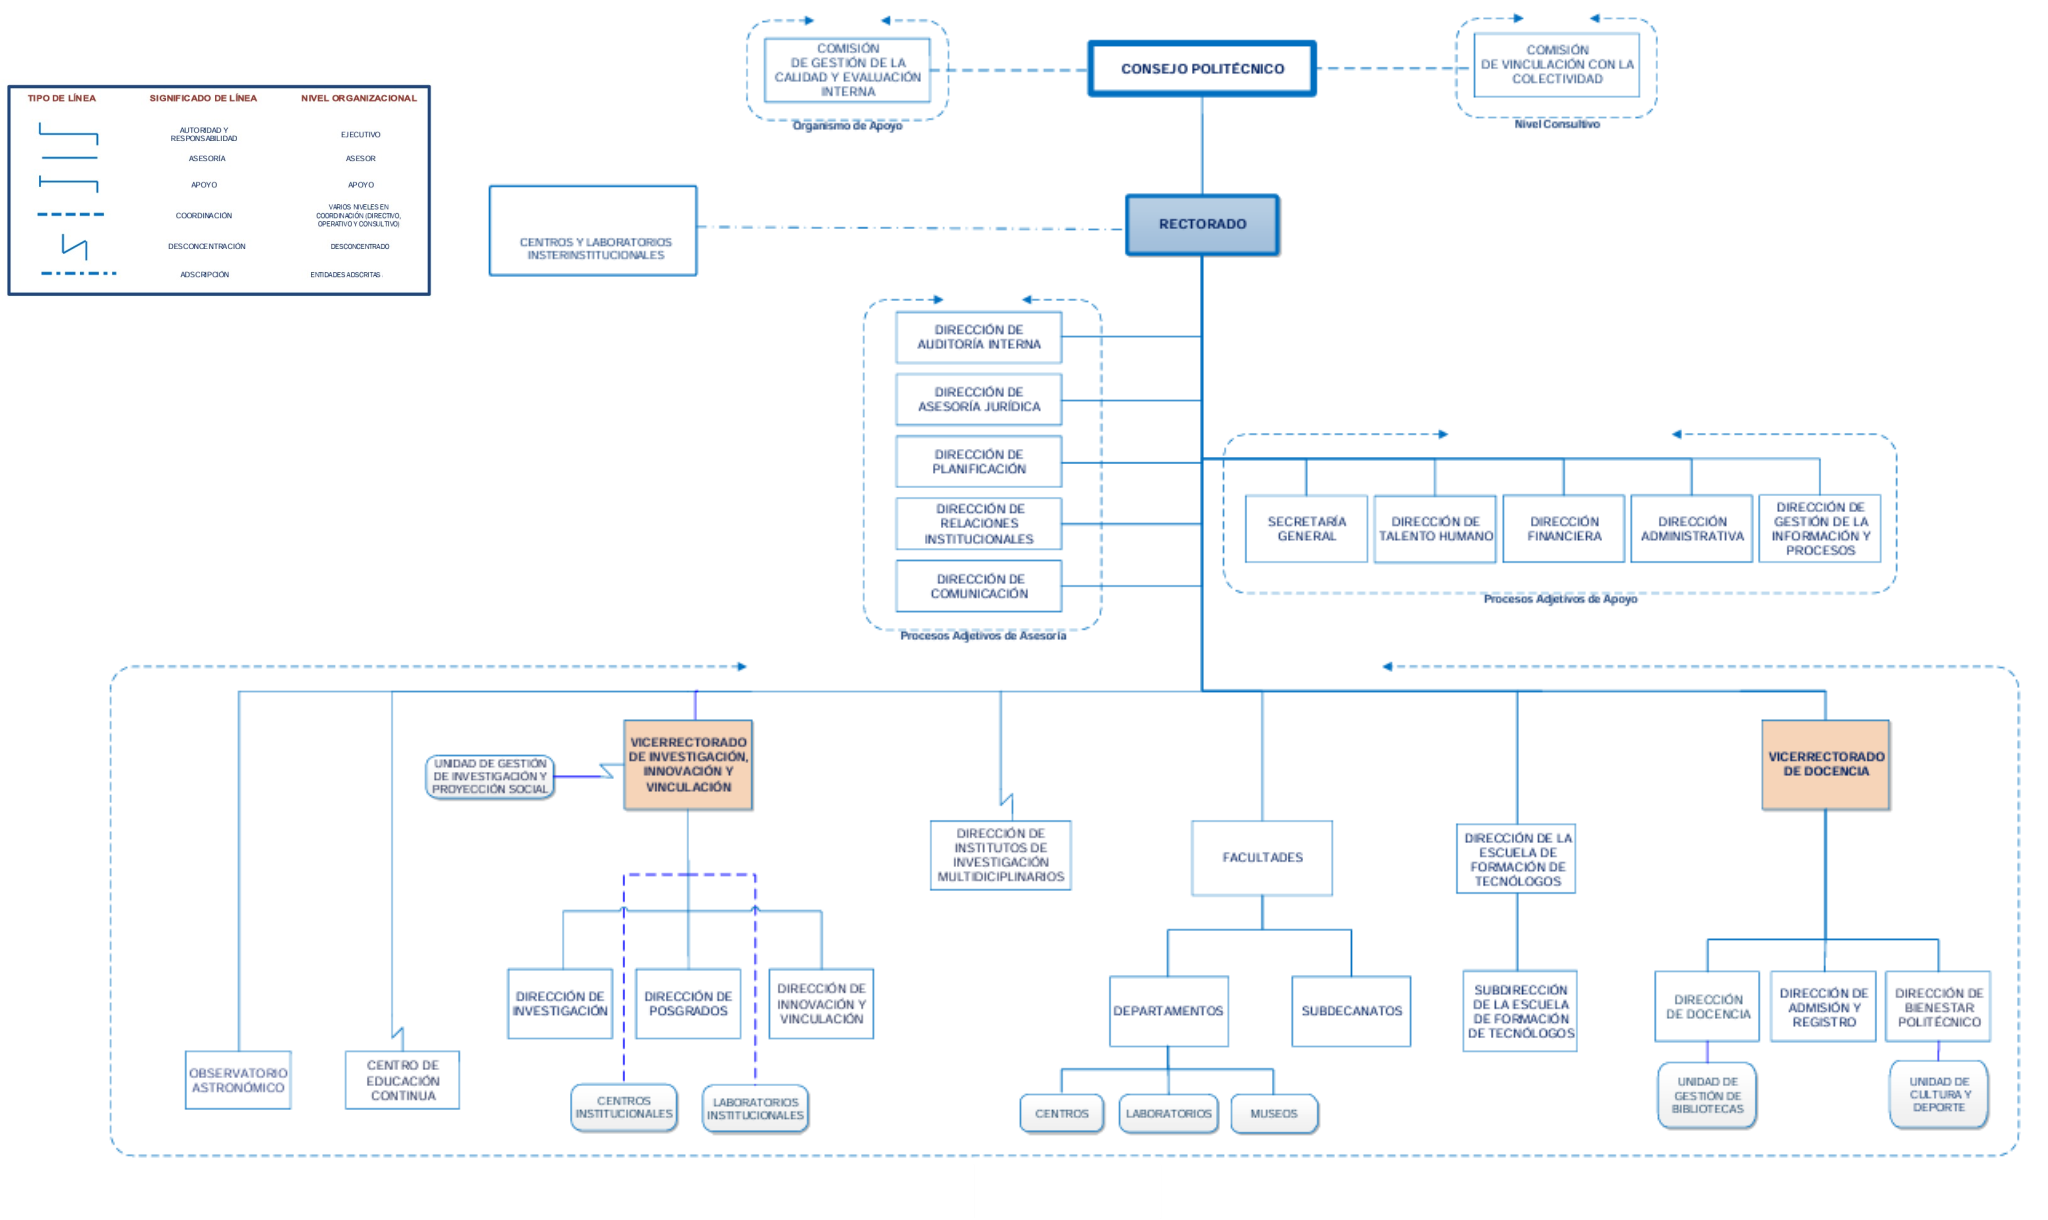
\includegraphics[width=0.9\linewidth]{images/Organigrama Universidad} \end{center}

Tomando como referencia el organigrama anterior se estima un universo
total aproximado de \emph{8.000 personas}, distribuidas entre
autoridades, docentes, personal administrativo/técnico y estudiantes.
Sin embargo, aplicando una \emph{tasa conservadora de participación del
15\%}, coherente con estudios institucionales similares, se proyecta un
total de: \emph{8.000 × 0.15 ≈ 1.200 encuestas válidas}.

\end{document}
